\chapter{Iteration 1}
\label{it:1}
\section{Planning}
This iteration revolved around setting up the back-end server and adding basic unit tests to the plugin. Aberystwyth authentication for staff (and potentially students) will be a major stepping stone for this sprint. Below is the list of stories and their assigned story points. The list is displayed in completion order.

\begin{itemize}
\item Add external change algorithm to find the difference: 2 points
\item Investigate testing framework for IntelliJ Plugin: 2 points
\item Write a test for copy-paste detection: 1 point
\item Write external change detection test: 2 points
\item Investigate server authentication: 3 points
\item Investigate data submission method: 2 points
\item Investigate back-end server software: 3 points
\item Docker support for quick deployment: 2 points
\item Implement web server: 1 point
\item Add database storage: 2 points
\item Implement server authentication: 2 points
\item Check if user is staff or student: 2 points
\item Add dashboard bootstrap template: 1 point
\end{itemize}

\section{Implementation}
\subsection{Implementing the External Change Detection Algorithm}
At the end of the last sprint, the external file change detection was implemented in the plugin. This needed an algorithm implemented to check the differences between the old and new file content. This requires a complex algorithm. After researching, the \textit{Myers' diff algorithm} was exactly what was needed. Originally, a third-party library implementation was going to be used, but IntelliJ already includes difference comparisons in the IDE. The SDK provides this functionality too. Albeit difficult at first, due to minimal documentation or examples provided. The \texttt{ComparisonManagerImpl} class provides methods to compare the characters between two strings and returns a list of \texttt{DiffFragments}. After converting these to a list of \texttt{Changes}, they were added to the appropriate \texttt{FileTracker} instance.

\subsection{Testing the Plugin}
The options for adding units tests to the plugin were limited to one choice. Due to the plugin being written in Java, JUnit was chosen. The IntelliJ Plugin SDK also provides an API for testing. The testing infrastructure provided by the SDK allows running tests in a headless environment. This means that the plugin can be tested without the UI while keeping the full functionality of the IDE. Despite the absurdly long class name, \texttt{LightPlatformCodeInsightFixtureTestCase}, provides the basics for unit tests with the IntelliJ Plugin SDK. Extending from \texttt{LightPlatformCodeInsightFixtureTestCase}, the \texttt{BaseTest} class was built to contain all of the useful testing methods for the plugin. This included methods such as \texttt{assertChangeListSize} and \texttt{assertOneChangeMatches}. The former method tests that the list of changes for a given file path is of a certain size. The latter method tests that the list of changes for a given file path contains a matching \texttt{Change} which is validated by the \texttt{Predicate}.

Extending from the \texttt{BaseTest} class, a test class for copy-paste detection was to be developed. This class contains one method which tests that when the clipboard is used to paste contents into the editor, it is identified properly. The testing infrastructure allows a file to be created in the test project, then a string value can be added to the clipboard and the editor can paste the clipboard contents. This data gets tracked as usual and then the file changes are tested against to verify that it was identified from the clipboard.

The second testing class added was to test the external file change detection. This is more complex than the simple copy and paste detection test. The project needs to be closed and the file must then be changed. This proved to be quite the challenge. To achieve this, originally, the project was actually closed but this prevented any files to be editable in the project. Instead, the \texttt{ProjectDocumentListener} which tracks all the file changes, was notified of the project closing, but the project would not be closed. Upon the project closing, the listener is removed from the project and file changes are not longer tracked. This allowed files to be editable, and in turn, would mimic external file changes. The \texttt{ProjectDocumentListener} was then notified that the project is opened and so the external changes would be detected and verified.

\subsection{Adding Authentication to the Server}
Prior to the development of the back-end server, the authentication mechanism was to be investigated. A member of IMPACS (Institute of Mathematics, Physics and Computer Science) was contacted about authentication via Aberystwyth University. This would allows staff and students to authenticate with the back-end server using their Aberystwyth credentials. This would minimise the amount of development needed for an independent authentication system. It would also remove the need for users to register with the new system. Instead, utilising the Aberystwyth LDAP (Lightweight Directory Access Protocol) server, users can be authenticated using their Aberystwyth University credentials. After the LDAP3 server details were acquired, this could be tested and verified. The back-end server is to be written in Python 3. The LDAP3 library provides the necessary API to connect to the Aberystwyth University LDAP server\cite{LDAP3Docs}. Following the documentation, a simple authentication method was developed to test the authentication functionality. Using the LDAP3 library, an LDAP server was created with a new connection for each user. Attempting to \texttt{bind} to connection would result in either success or failure. If the bind was successful, then the user is authenticated and further user information may be retrieved from the connection.

\subsection{Deciding on the Server Submission Method}
Before continuing development on the back-end server, the data submission method must be decided. This is the choice of either the continuous or non-continuous back-end server. The \nameref{sec:analysis} contains details on both of these methods. In the end, the non-continuous server was chosen. This is due to the simplicity of the design. It provides better support for offline development, and students will not be required to interact with the plugin. However, the server will have to provide authentication for both staff and students, as well as separate user interfaces for both. Students will also have to submit their tracked data via the user interface but this should be less complex than continuously sending the data through a network protocol.

\subsection{Parsing and Storing the XML Data}
Now that the chosen authentication method is implemented and the data submission method has been chosen, the back-end server development can continue. The back-end server will need to parse the tracked XML data file. The database being used to store the tracked data is MongoDB which is a NoSQL database. The parsed XML data will need to be transformed into a JSON-like document. This didn't prove difficult due to the similarities between the structure of JSON and XML.

Using the \texttt{xml.etree.ElementTree} module, the XML data was parsed. But due to the format that the \texttt{PersistentStateComponent}, the XML parsing needed a little more intelligence. The XML data contains nested lists in a map, so these data structures would need to be correctly parsed. Recursively iterating over each element in the XML tree, each element was processed depending on its data. If the element was a map, then its children would be parsed as key-value pairs. If the element was a list, then its children would be added to a list. Any other element was parsed with a name and a value. All elements were added to a dictionary. Each element is guaranteed to have a name due to the serialisation assigning names to each element for each field.

For MongoDB, the PyMongo library was used to interface with the database connection\cite{PyMongoDocs}. Following the documentation, the tutorial was simple enough to follow to setup a connection to a local MongoDB instance. The \texttt{SubmissionCollection} class was written to provide useful database methods. Primarily, these methods are used to find, and insert data into the database easily. \nameref{sec:mongodb-student-document} in \nameref{chp:code-examples} shows the document data structure for a typical user.

\subsection{Using Flask to Deliver Web Content}
The back-end server must provide a service to staff and students. Enter, Flask. Flask provides a micro web framework. Flask uses function decorators to specify URL routes. The return value of the function is then displayed when requested. Flask uses a templating language known as Jinja2. Jinja2 allows HTML templates to be dynamically rendered for each request. Pairing the templates with Bootstrap and JQuery allows to present beautiful dynamic web pages for end users. The front-end web application doesn't do much currently. The end users must be able to login using their Aberystwyth University credentials. To combine LDAP server authentication with Flask seamlessly, we need another library; Flask-Login.

Flask-Login provides user session management for Flask. Using the Bootstrap sign-in template\cite{BootstrapSignInTemplate} and Flask-Login, the authentication system worked perfectly. A single route was used for the index. The index renders the sign-in template when using the GET request. This is shown in \autoref{fig:web-sign-in}. However, when a POST request is sent, authentication is performed using the posted form values (username and password). The username and password are used for binding a new LDAP connection. Upon success, the user details are retrieved from the LDAP server and a new user model is created using the User class. The User class follows the model from Flask-Login providing the required methods. An additional method has been added to test if the user is staff. The user details are stored in the database. If the user already exists in the database, then an update is triggered instead. This will update and out-of-date details. The page is then redirect to the appropriate dashboard. Staff and students have separate dashboards. If authentication is unsuccessful then a flash message is displayed to the user and the sign-in page is displayed. This is shown in \autoref{fig:web-sign-in-invalid}

\begin{figure}[H]
  \centering
  \fbox{
    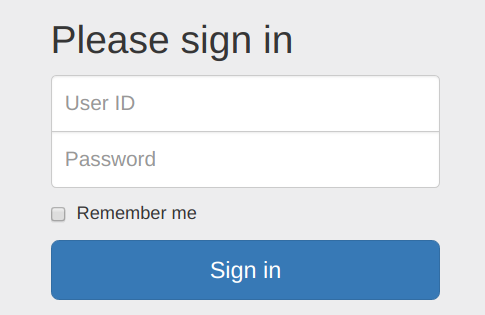
\includegraphics[height=.6\textheight,
    keepaspectratio=true,
    width=.6\textwidth,
    ]{figures/05-web-sign-in.png}
  }
  \caption[Web Sign-in Page]{The index page of the web-application. This is where users sign-in.}
  \label{fig:web-sign-in}
\end{figure}

\begin{figure}[H]
  \centering
  \fbox{
    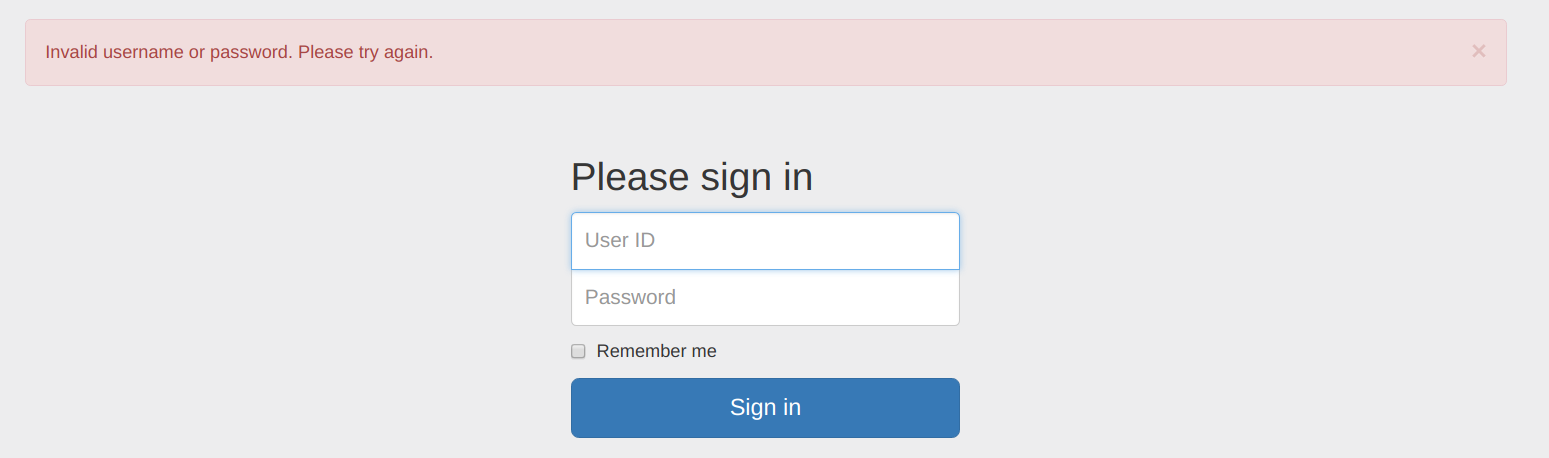
\includegraphics[height=\textheight,
    keepaspectratio=true,
    width=\textwidth,
    ]{figures/06-web-sign-in-invalid.png}
  }
  \caption[Web Invalid Sign-in Flash]{An error flash message is displayed when a user enters incorrect credentials on the sign-in form.}
  \label{fig:web-sign-in-invalid}
\end{figure}

\subsection{Dockerising the Server}
Docker is a software technology providing containers. Docker provides base images or operating systems, such as Ubuntu which can be downloaded and run out of the box. Docker also allows images to be built in layers, meaning that developers can build on top of these base images and distribute their images (which can then be used as base images for others to download). A Dockerfile is a text file which contains commands to build an image. This allows for seamless automation of building Docker images and running Docker containers. A \texttt{Dockerfile} was created for the back-end server. This will install all of the required python packages using pip. The base image used is \texttt{python:3.6.4-slim}. This provides the basic Python infrastructure. All of the required files are added to the container upon running the container by mounting the directory to a volume in the container. Another \texttt{Dockerfile} was written for the MongoDB instance. The \texttt{docker-compose.yml} file is used by Docker Compose to run multiple-container applications. This allows deployment of the containers (back-end server, and MongoDB) with one command; \texttt{docker-compose up} to start, and \texttt{docker-compose down} to stop.

\section{Retrospective}
The velocity for this sprint is 25. This is a large increase from the first sprint. Again this sprint had bad estimates for stories. Initially, the sprint ended prematurely, so more stories were added to accommodate this. Alternatively, the sprint could've been closed and a new one started. Aside from the bad estimations, the work completed during this iteration was comprehensive.
